\section{CosmoScout VR}\label{sec:cosmoscout-vr}

\begin{wrapfigure}{o}{0.5\textwidth}
    \centering
    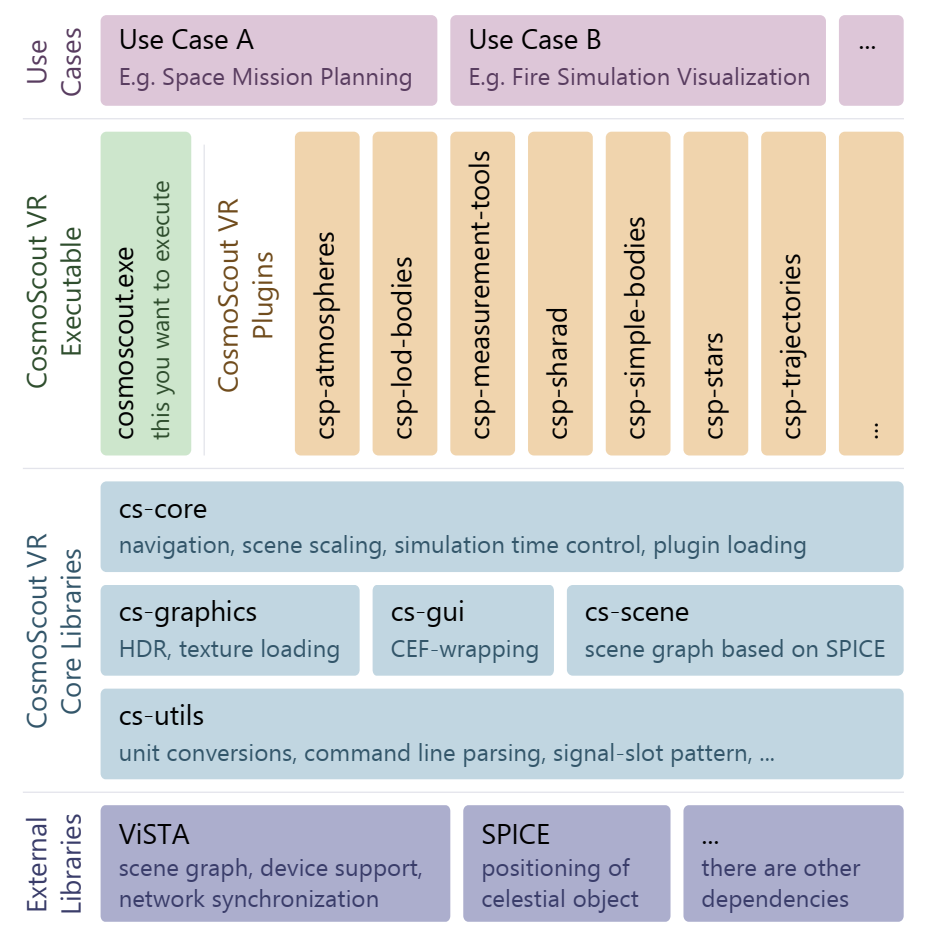
\includegraphics[width=0.5\textwidth]{content/2_3_cosmoscout/img/cosmoscout-architecture}
    \caption{CosmoScout VR architecture~\cite{CSVR}.}
    \label{fig:cosmoscout-architecture}
\end{wrapfigure}

Cosmoscout VR is a modular, scientific, 3D visualisation of the solar system, with the goal to provide interactive,
and immersive exploration of large datasets.
Recent earth observation and space exploration in the international community has produced vast amounts of data at a
scale that can be difficult to process and visualise.
CosmoScout VR has the goal of visualising these increasingly large datasets at diverse scales, with the virtual
environment allowing natural, and intuitive interaction, and explorative analysis of the data.

CosmoScout VR uses a modular, layered architecture to provide high-flexibility for different use cases.
The basis is composed of five core libraries that provide basic functionalities, using external dependencies to
realize key components, like ViSTA for the scene graph, and network synchronization, and SPICE for precise positioning
of celestial objects.
The core libraries are used in the slim executable, that is packaged with a modular collection of Plugins, providing
the key functionality of CosmoScout VR, while the Plugins can still be customized to focus the application for
specific use cases.
